
Der Spielzeitenplaner ist grundsätzlich in vier verschiedene Bereiche eingeteilt: 
Team, Recap, Spielzeiten planen und Einstellungen. Diese Bereiche und die damit 
verbundenen Grundfunktionen des Spielzeitenplaners sollen im Folgenden kurz 
beschrieben und erläutert werden. \\ 
Als Erstes ist der Team-Bereich zu nennen, der sich im Wesentlichen aus zwei Teilen 
zusammensetzt: der Team-Seite und der Spieler-Seite. Auf Ersterer lässt sich ein 
Teamname festlegen und speichern oder ändern. Außerdem wird eine Liste mit allen 
Spielern im Team und den dazugehörigen Daten (Name, Position, Trikotnummer, etc.) 
angezeigt (siehe Abbildung 1). \\ 
In der aktuellen Version des Spielzeitenplaners wird sich 
zunächst auf nur ein Team beschränkt, da ein Großteil aller Fußballlehrenden nicht in 
mehreren Teams zugleich aktiv ist. Eine Unterstützung mehrerer Teams ist jedoch in 
zukünftigen Versionen bereits eingeplant. Darüber hinaus sind Persistenz- und 
Service-Schicht bereits im Hinblick auf die Verwendung mehrerer Teams entsprechend 
ausgelegt worden oder es sind nur kleinere Änderungen notwendig, um diese Funktionalität 
künftig unterstützen zu können. \\ 

\begin{figure}[h]
  \centering
  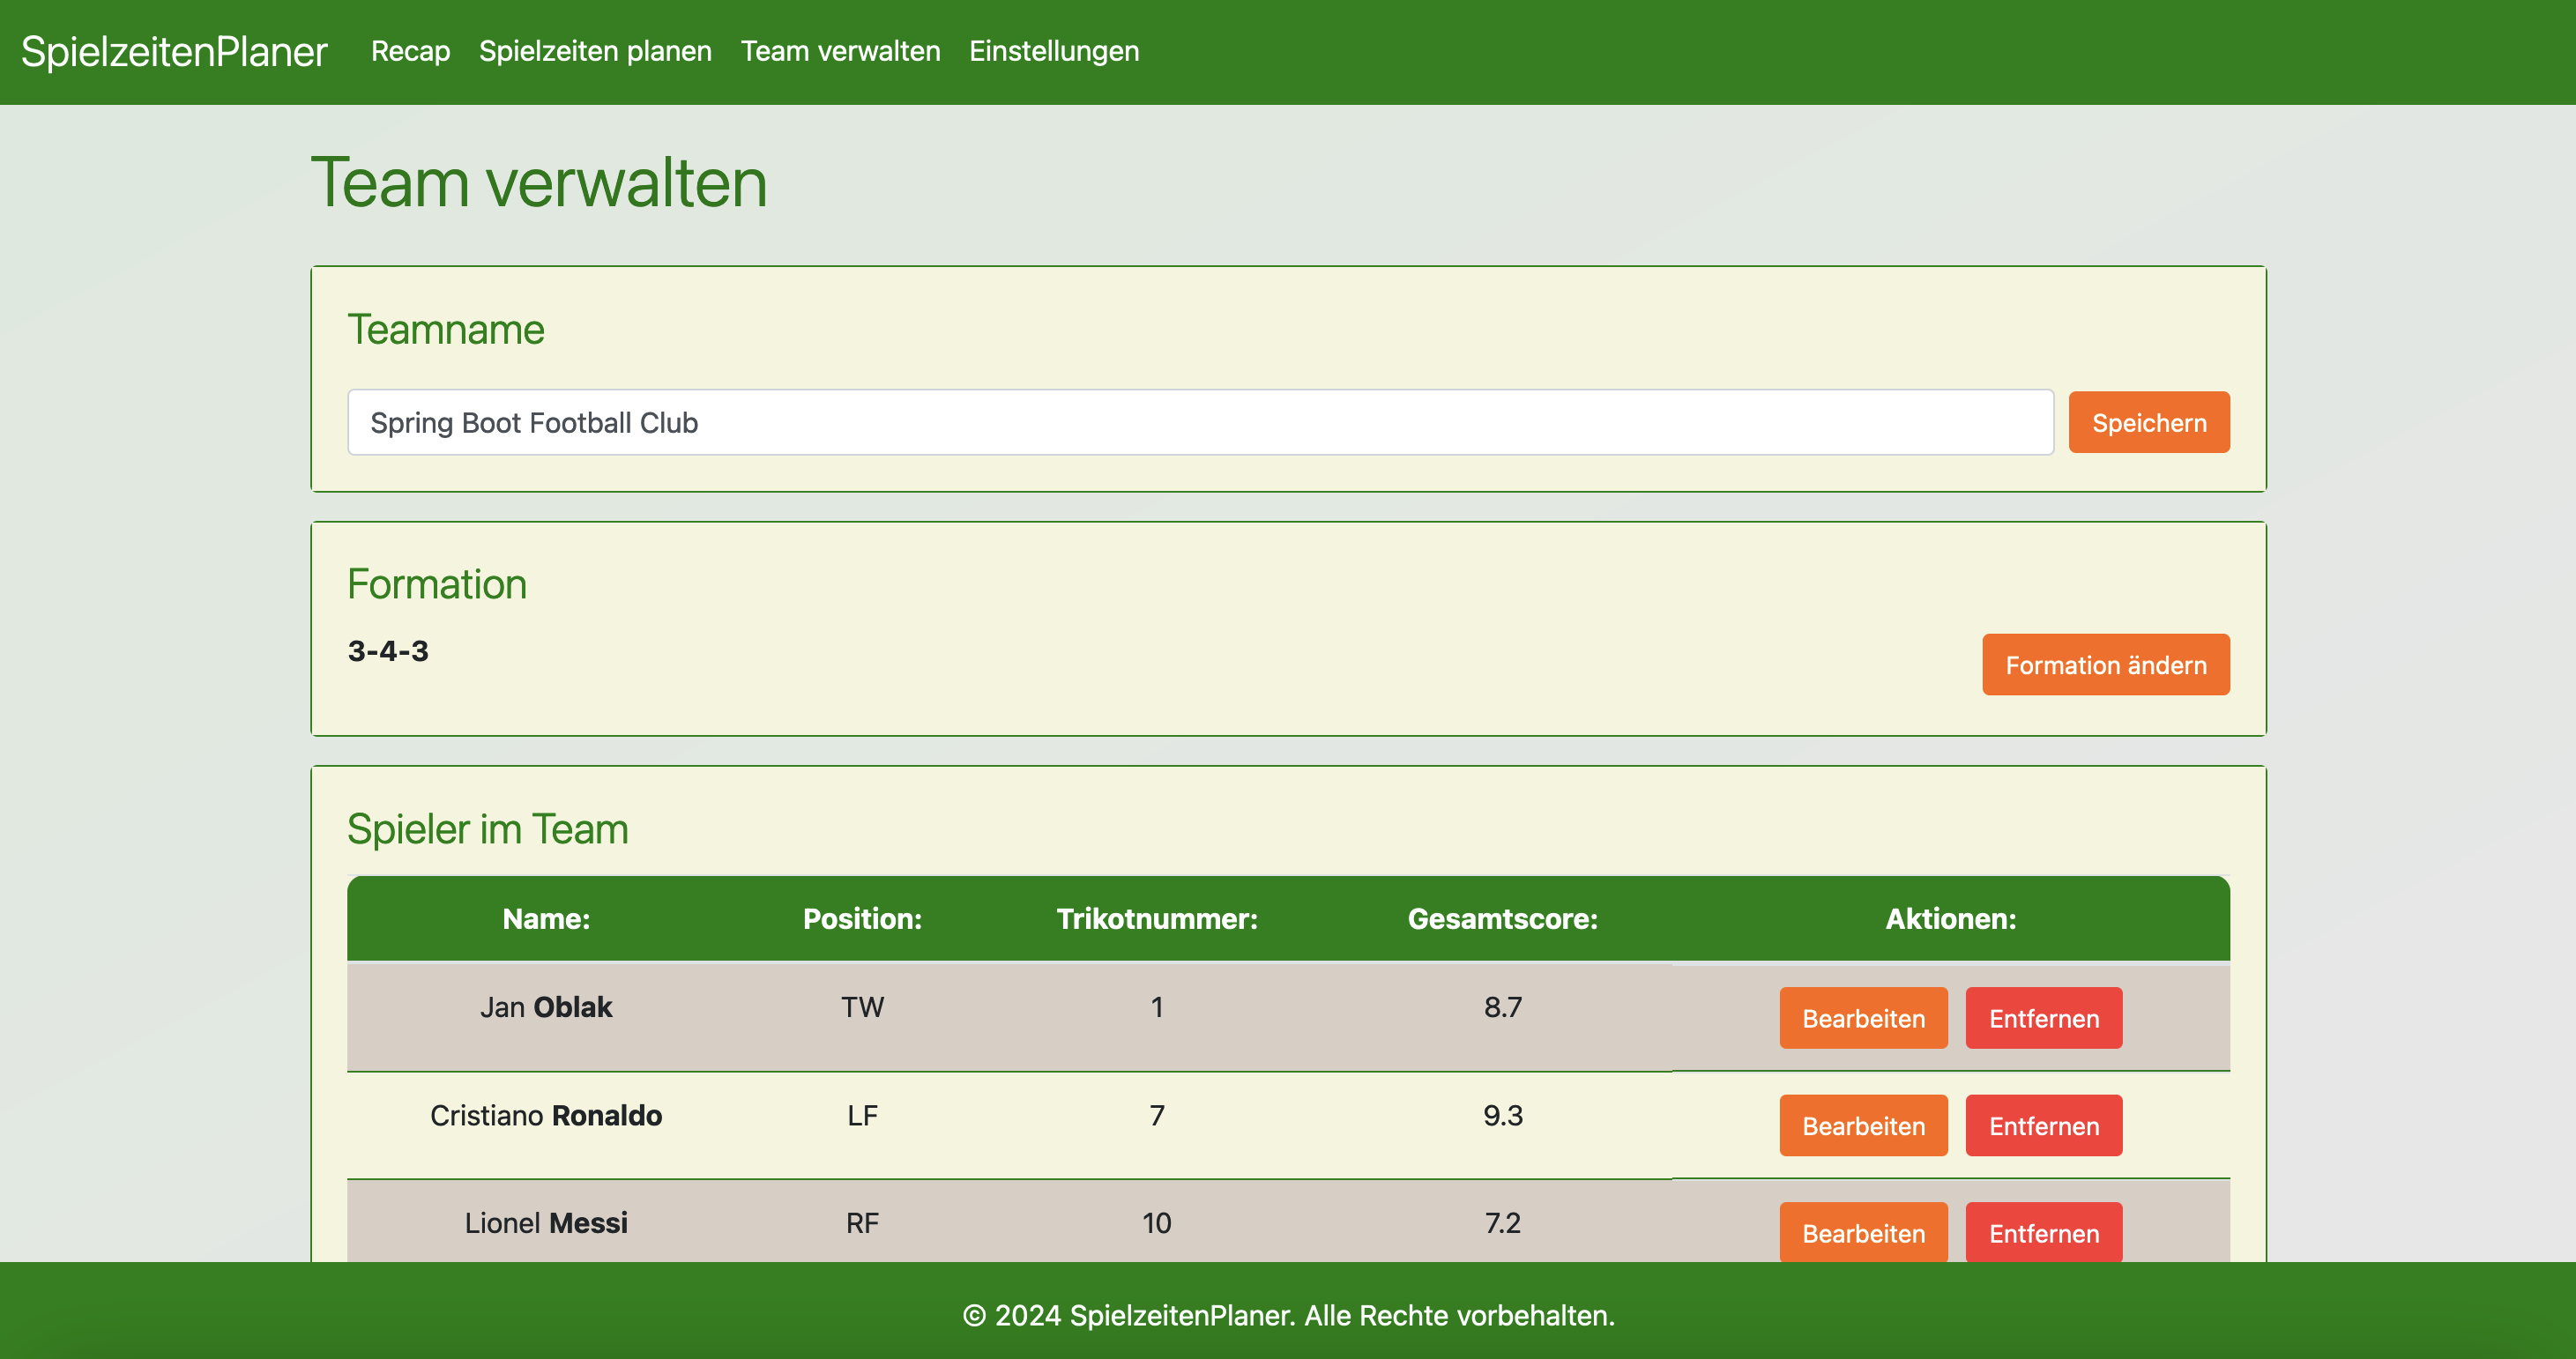
\includegraphics[width=\textwidth]{screenshots/teampage.png}
  \caption{Screenshot der Team-Seite}
  \label{fig:teampage}
\end{figure}

Für jeden Spieler gibt es die Möglichkeit, diesen entweder zu bearbeiten oder zu löschen. 
Mit einem Klick auf den Löschen-Button wird der entsprechende Spieler gelöscht, durch den 
Klick auf den Bearbeiten-Button hingegen gelangt man zur Spieler-Seite. \\ 
Diese enthält sowohl die individuellen Spieler-Daten des aktuell ausgewählten Spielers 
wie auch eine Anzeige der Spieler-Scores. Hier können Vor-, Nachname, Position und 
Trikotnummer des ausgewählten Spielers geändert werden. Wählt man auf der Team-Seite den 
Button zum Erstellen eines neuen Spielers, so wird die Spieler-Seite mit einem leeren 
Formular aufgerufen, sodass ein neuer Spieler erstellt und anschließend gespeichert 
werden kann. \\ 
Der Bereich Einstellungen enthält -- wie der Name bereits suggeriert -- einige 
grundsätzliche Einstellungen, die insbesondere für den Bereich des Planens der 
Spielzeiten von Bedeutung sind. Unter anderem besteht hier die Möglichkeit, eine 
eigene Formation zu erstellen. Dafür sind die Angabe eines Namens -- zum Beispiel 
\textit{4-4-2} oder \textit{3-4-3} -- sowie die Bezeichnungen der einzelnen 
Positionen notwendig (siehe Abbildung 2). Dabei werden diese geordnet von hinten nach 
vorne (Torwart, Verteidigung, Mittelfeld, Sturm) sowie von links nach rechts (linker 
Flügel, Zentrum, rechter Flügel) angegeben. \\ 

\begin{figure}[h]
  \centering
  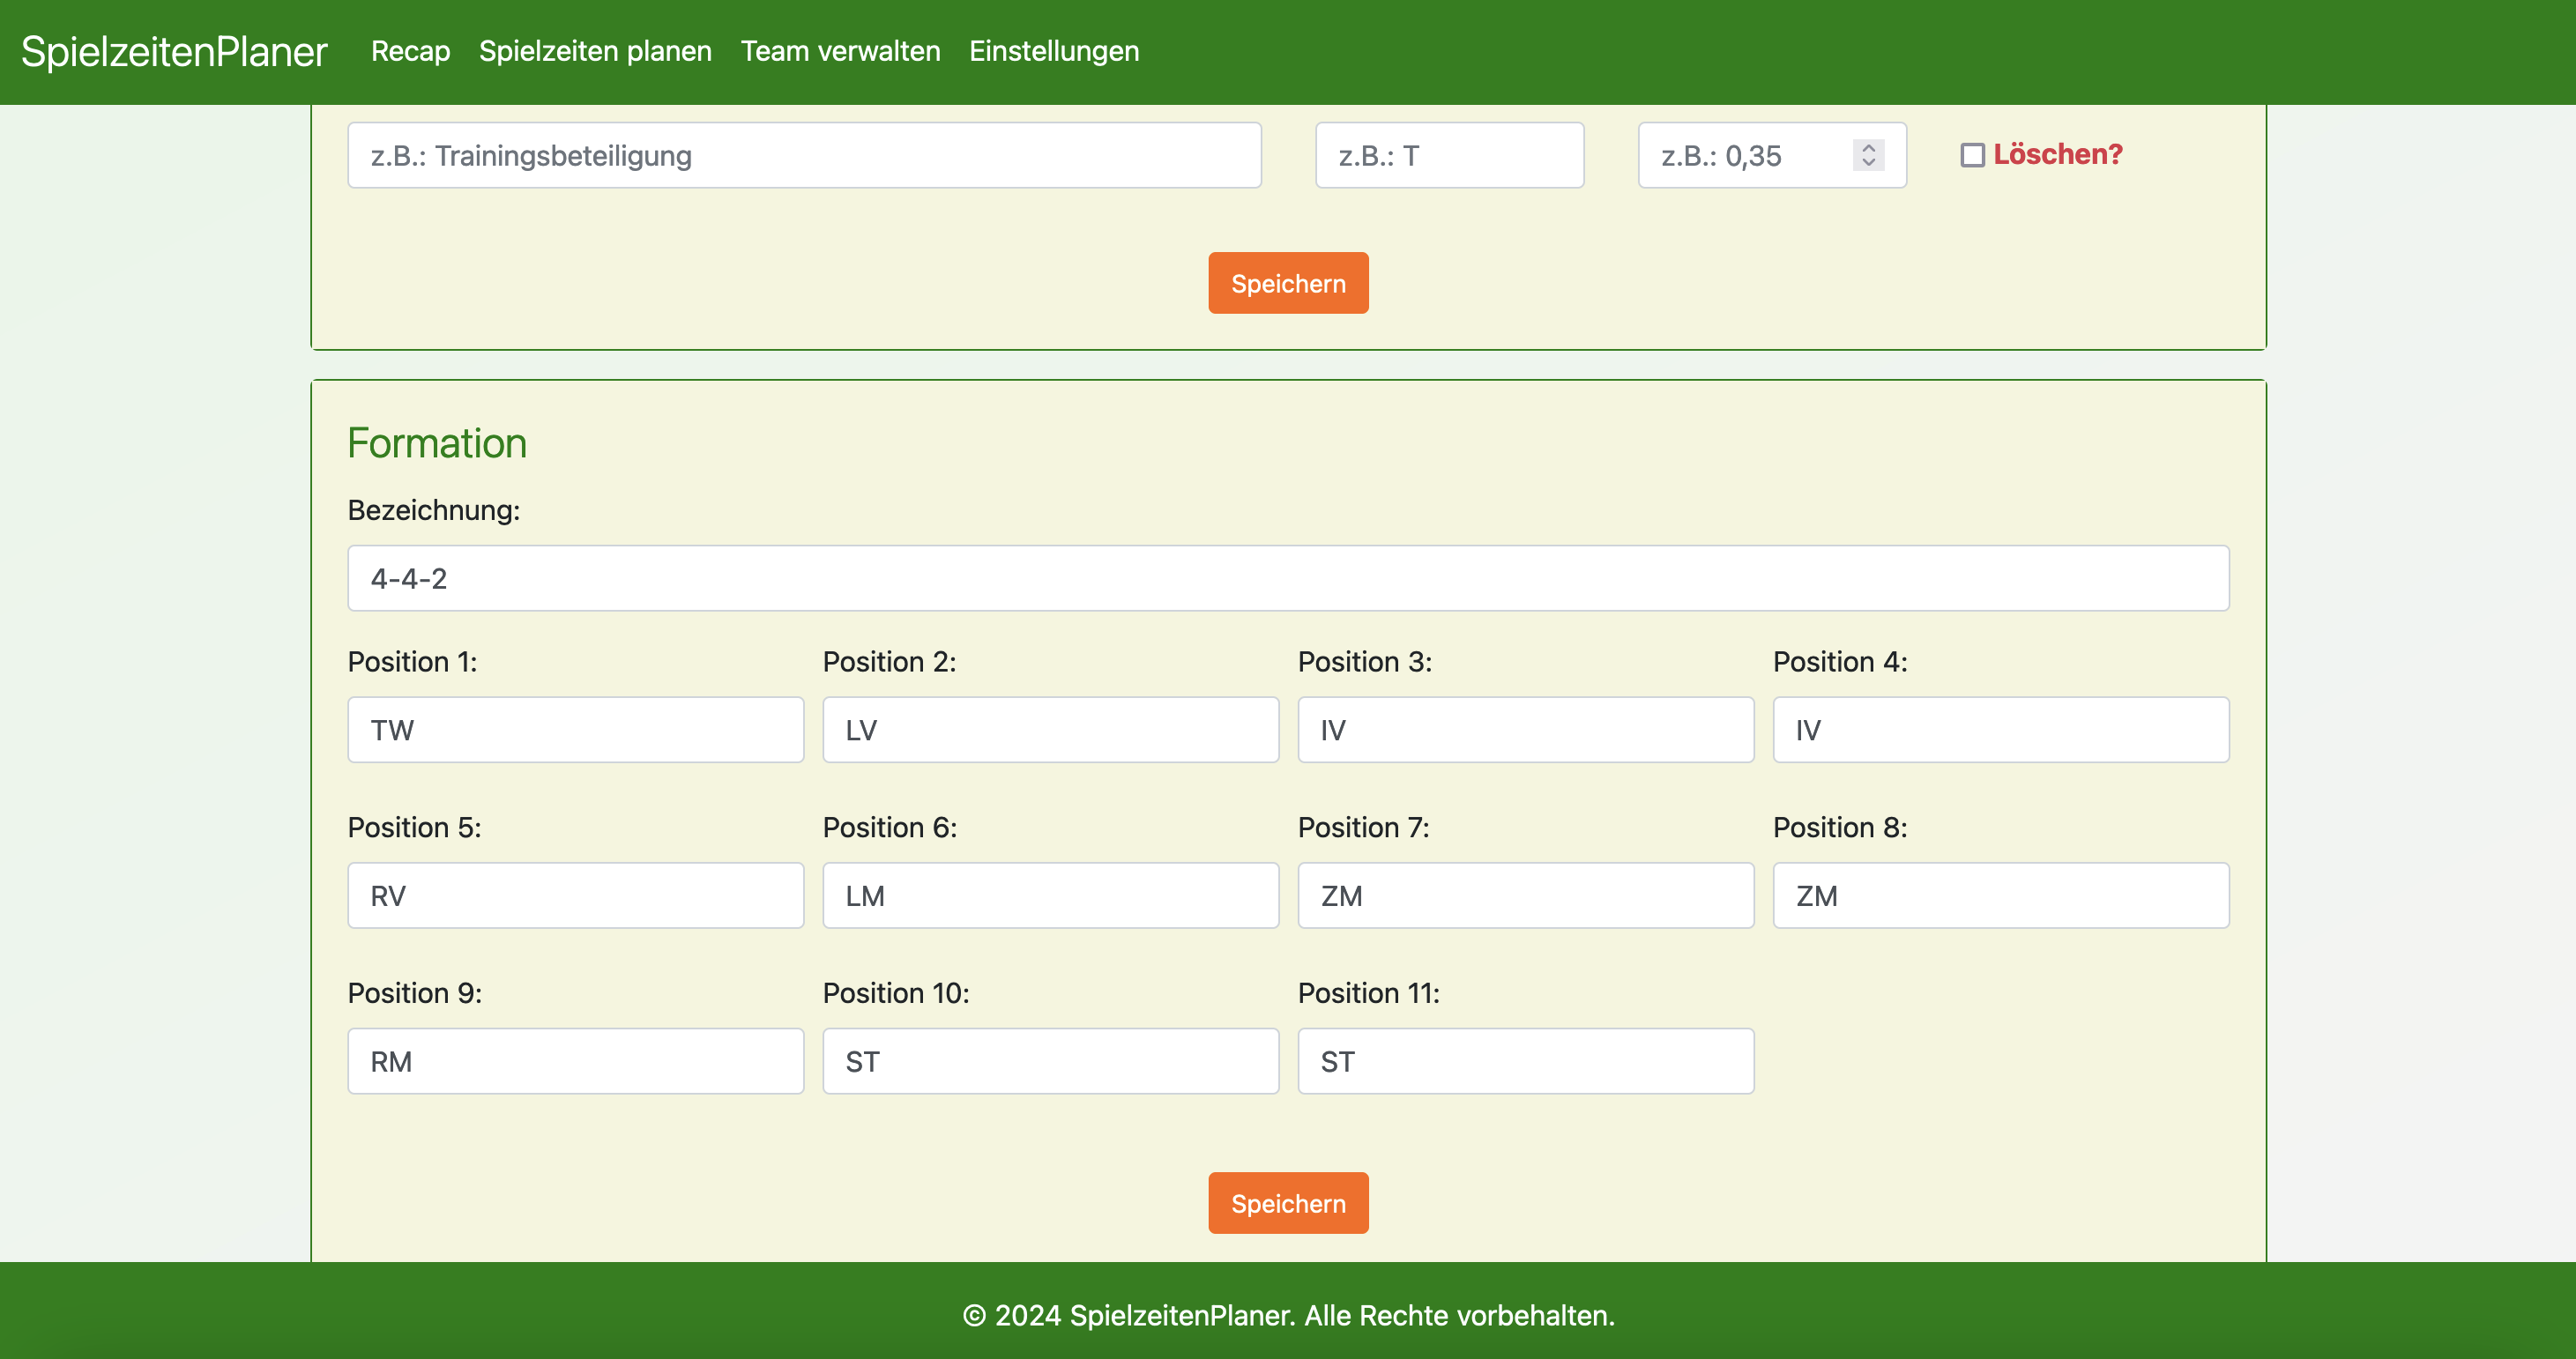
\includegraphics[width=\textwidth]{screenshots/formation.png}
  \caption{In den Einstellungen lässt sich die Formation bearbeiten/speichern}
  \label{fig:formation}
\end{figure}

Über dem Abschnitt zur Formation befindet sich der Kriterien-Abschnitt. Hier können 
Kriterien erstellt, bearbeitet und gelöscht werden. Diese sind von zentraler 
Bedeutung bei der Bewertung der Spieler im Recap-Bereich. Für die Erstellung eines 
Kriteriums wird ein Name bzw. eine Bezeichnung, eine Abkürzung (ein bis zwei 
Buchstaben) und eine Gewichtung benötigt. Die Summe aller Gewichte sollte stets 
eins ergeben, ein einzelnes Gewicht im Bereich zwischen null und eins liegen. 
Die wohl gebräuchlichsten Kriterien sind zum Beispiel die Trainingsbeteiligung und 
die Leistung. \\ 
Schließlich gibt es noch die Scores-Einstellungen, die ganz oben auf der Seite 
zu finden sind. In diesem Bereich lässt sich der Zeitraum festlegen, auf dessen 
Grundlage die Scores für die einzelnen Kriterien berechnet werden. Für das 
Kriterium der Trainingsbeteiligung gibt es zusätzlich noch besondere Einstellungen: Zum 
einen kann zwischen einer kurzfristigen und langfristigen Trainingsbeteiligung 
unterschieden, zum anderen können spezifische Gewichte für die Kurz- und Langfrist 
festgelegt werden. \\ 
Folgendes Beispiel soll zur Verdeutlichung des Sachverhaltes herangezogen werden: 
Ein Trainerteam entscheidet sich dazu, dass die Trainingsbeteiligung 50 Prozent 
des Gesamt-Scores ausmachen soll. Innerhalb der Trainingsbeteiligung wird dann 
nochmals festgelegt, dass die letzten drei Wochen für die Kurzfrist herangezogen 
werden sollen und die letzten acht Wochen für die Langfrist. Da das Trainerteam 
etwas mehr Wert auf eine langfristige Teilnahme am Training legt, werden die 
Gewichte auf $ 0.4 $ für die Kurzfrist und $ 0.6 $ für die Langfrist festgelegt. 
Somit berechnet sich der Score für dieses Kriterium zu 60 Prozent aus der 
langfristigen Trainingsbeteiligung und zu 40 Prozent aus der Kurzfrist. So kann 
ein Spieler, der grundsätzlich immer am Training teilnimmt, ein kurzfristiges 
Fehlen aufgrund von Krankheit oder schulischer Verpflichtungen durch einen hohen 
Score in der Langfrist korrigieren. \\ 
Der dritte große Bereich der Anwendung ist das Recap. Im Wesentlichen geschieht 
hier Folgendes: Nach jedem Training wird eine Bewertung eines jeden Spielers zu jedem 
Kriterium vorgenommen. Die Bewertungen werden gespeichert und zur Ermittlung der 
Scores für jedes Kriterium sowie des Gesamtscores herangezogen. Letzterer wiederum 
ist von wesentlicher Relevanz bei der Planung der Spielzeiten -- also der 
Spielminuten -- für das kommende Spiel. Um zur Recap-Seite zu gelangen, werden in 
einem ersten Schritt all diejenigen Spieler ausgewählt, die am Training 
teilgenommen haben. Diese Information wird dann auf der eigentlichen 
Bewertungsseite genutzt, um eine Vorsortierung der Spieler vorzunehmen. \\ 

\begin{figure}[h]
  \centering
  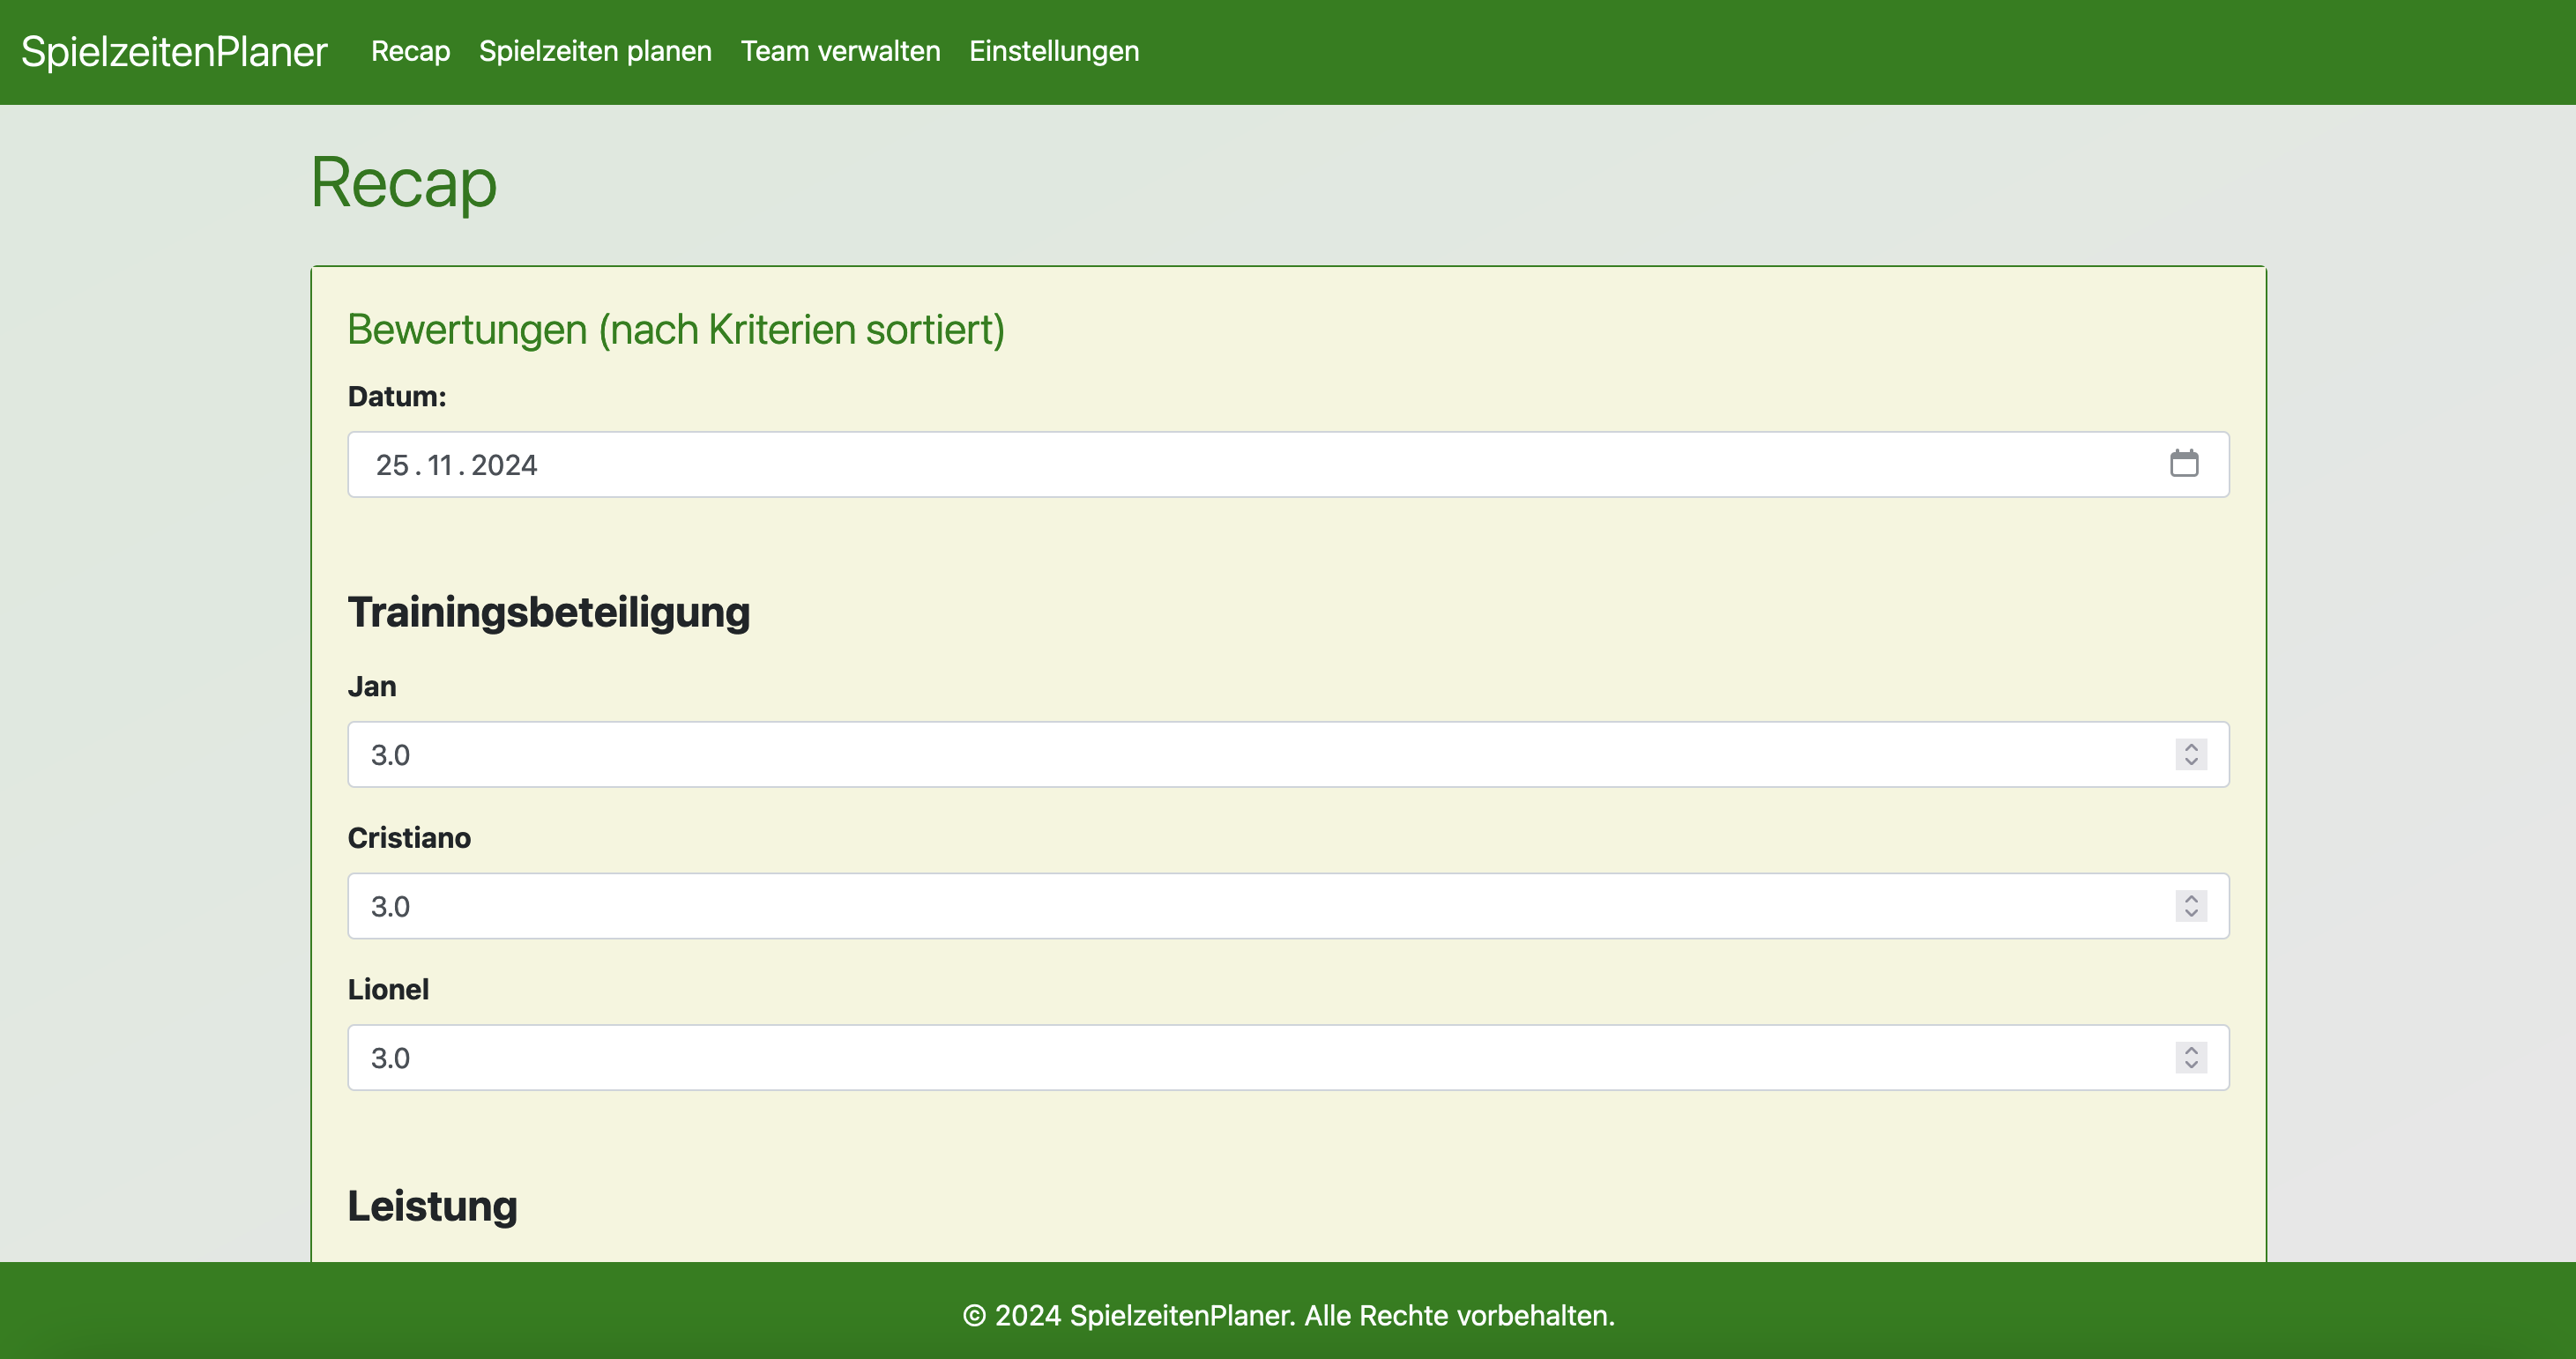
\includegraphics[width=\textwidth]{screenshots/recap.png}
  \caption{Auf der Recap-Seite wird jeder Spieler bewertet}
  \label{fig:recap}
\end{figure}

Grundsätzlich ist die Recap-Seite nach den vorhandenen Kriterien 
gegliedert, das bedeutet, dass für jedes Kriterium eine Liste mit Spielern 
angezeigt wird, für die dann eine Bewertung abgegeben wird (siehe Abbildung 3). Die 
Bewertung erfolgt auf einer Skala von eins bis fünf, wobei eine Drei den Durchschnitt 
bildet, eine Eins eine deutlich unterdurchschnittliche Bewertung darstellt und eine Fünf 
die bestmögliche Bewertung ist. Dementsprechend ist eine Vier als tendenziell 
überdurchschnittlich und eine Zwei als tendenziell unterdurchschnittlich zu 
betrachten. \\ 
Da der jeweilige Wert serverseitig als Double abgebildet wird, ist es den Nutzenden 
möglich, weitere Abstufungen vorzunehmen, beispielsweise eine $ 2.5 $ oder 
$ 4.5 $ zu vergeben. Für eine schnelle und effiziente Bewertung ist es jedoch 
ratsam, bei den Bewertungen eins, zwei, drei, vier und fünf zu bleiben. Für einen 
Spieler, der beim Training nicht anwesend ist, wird standardmäßig eine $ 0.0 $ 
vergeben. Die Null-Bewertungen werden dann serverseitig herausgefiltert und 
nicht gespeichert, da ein häufiges Fehlen sonst nicht nur den Score der 
Trainingsbeteiligung, sondern auch alle anderen Scores verringern würde, was einer 
gleich mehrfachen Abwertung gleichkäme. \\ 
Schließlich ist dann noch der Bereich der Spielzeitenplanung zu nennen. Hier können 
die Nutzenden vor einem Spiel planen, wie viele Minuten Spielzeit jeder einzelne 
Spieler basierend auf dem Gesamtscore erhalten soll. Die Spielzeitenplanung 
gestaltet sich als ein mehrstufiges Verfahren, durch das die Nutzenden vom 
Spielzeitenplaner geleitet werden. \\ 
In einem ersten Schritt werden zunächst alle Spieler ausgewählt, die für das 
kommende Spiel zur Verfügung stehen, die also nicht krank oder verletzt sind oder 
aufgrund von privaten Terminen und anderen Gründen abgesagt haben. Aus den 
verfügbaren Spielern wird dann in einem zweiten Schritt ermittelt, welche Spieler 
es in den Kader geschafft haben und welche nicht. Die vorgeschlagene Aufteilung 
kann dabei übernommen oder aber manuell durch die Nutzenden überarbeitet werden, 
sodass das Trainerteam die Kontrolle über die Spielzeitenplanung behält. \\ 

\begin{figure}[h]
  \centering
  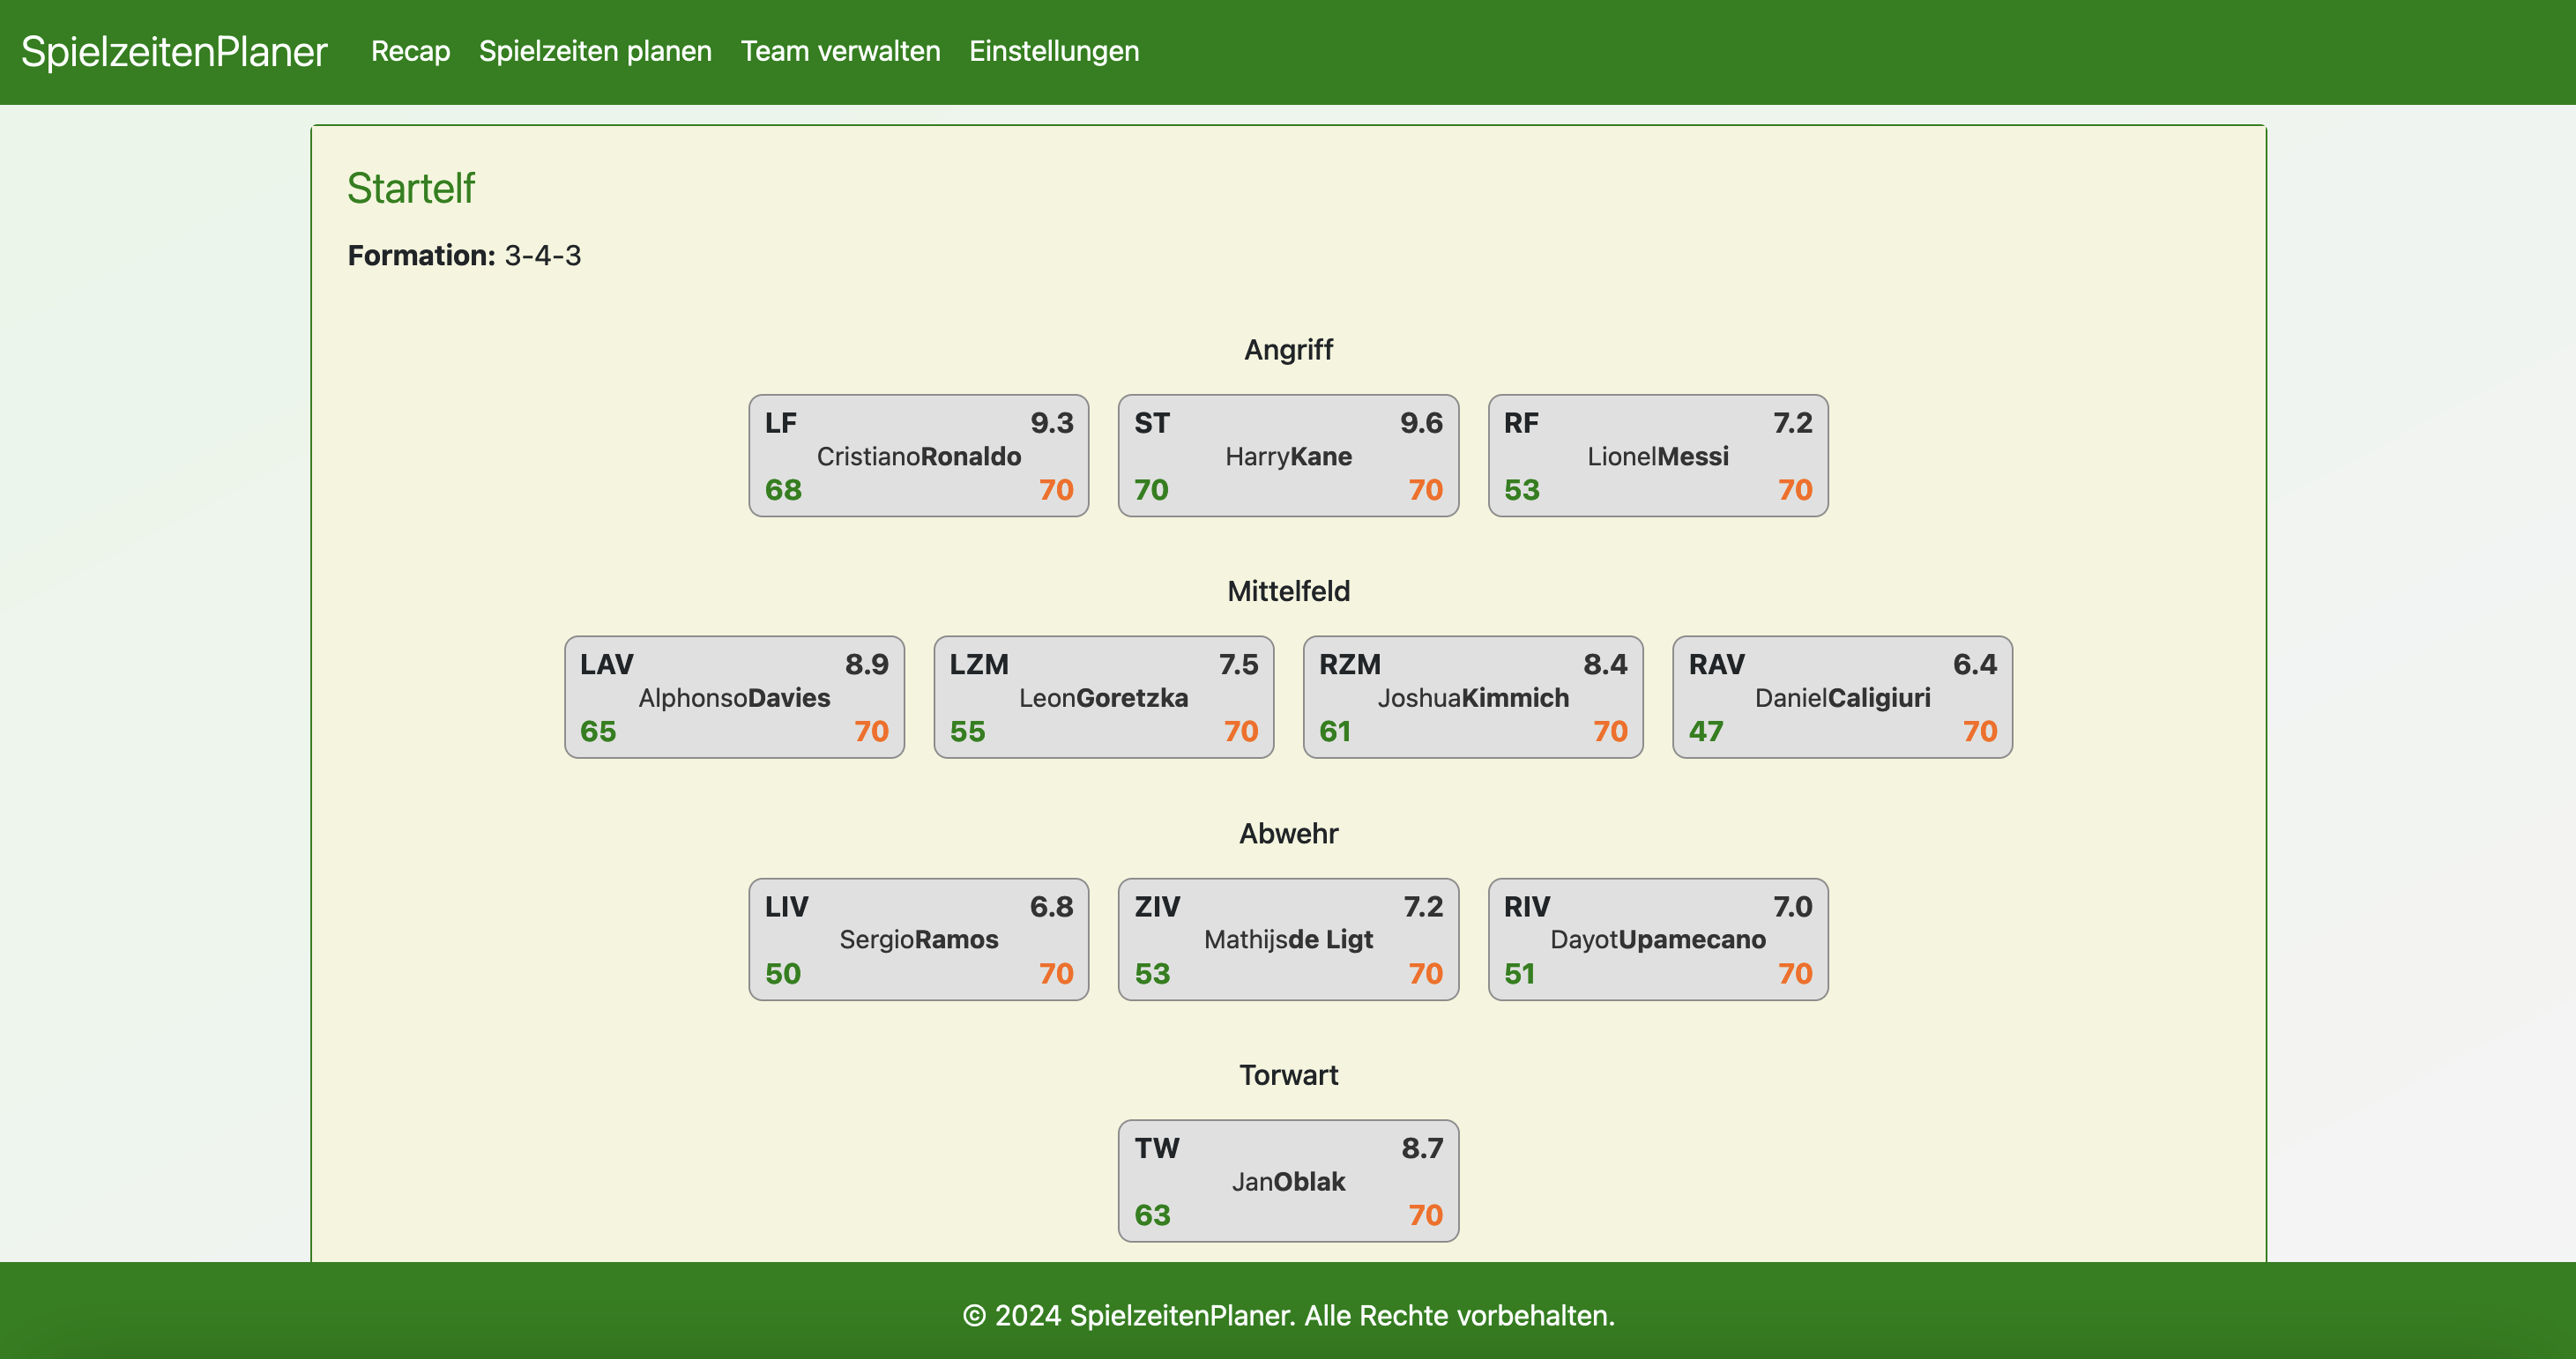
\includegraphics[width=\textwidth]{screenshots/spielzeiten.png}
  \caption{Startelf inklusive berechneter und geplanter Spielminuten}
  \label{fig:spielzeiten}
\end{figure}

\pagebreak

Nachdem der Kader feststeht und das entsprechende Formular durch die Benutzenden 
abgeschickt worden ist, wird in einem dritten Schritt aus dem Kader die Startelf 
bestimmt. Auch bei diesem Schritt können die Nutzenden Einfluss nehmen, indem 
Positionen getauscht oder Spieler von der Bank in die Startelf gesetzt werden. Ist 
die Startelf ermittelt, kommt es zum letzten Schritt der Spielzeitenplanung: 
dem Eintragen der Wechsel. Dieser letzte Planungsschritt ist essenziell für die 
Bestimmung der Spielzeiten, denn mit dem Feststehen der Wechsel bzw. der 
Wechsel-Zeitpunkte steht ebenfalls fest, welcher Spieler wie viele Minuten auf dem 
Platz steht (siehe Abbildung 4). \\ 
Wie bei den vorherigen Planungsschritten besitzen die Nutzenden auch hier die volle 
Kontrolle: sowohl Einwechsel- wie Auswechselspieler aber auch die konkrete 
Spielminute kann bestimmt werden. Die voraussichtliche Anzahl der Spielminuten für 
jeden einzelnen Spieler wird auf Basis der gespeicherten Wechsel berechnet und auf 
der Seite angezeigt. Außerdem wird vom Spielzeitenplaner eine erwartete Spielzeit 
berechnet. Diese errechnet sich maßgeblich aufgrund des Gesamtscores eines Spielers 
und stellt diejenige Spielzeit dar, die basierend auf den Bewertungen des 
entsprechenden Spielers als fair erachtet wird. \\ 
Nun können Nutzende so lange wie nötig Anpassungen vornehmen -- das heißt neue 
Wechsel eintragen, Wechsel löschen oder die Wechselzeitpunkte anpassen -- bis 
die voraussichtliche Anzahl der Spielminuten eines jeden Spielers ungefähr mit der 
Anzahl der erwarteten Spielminuten übereinstimmt. Ein weiteres Mal ist es dem 
Trainerteam selbst überlassen zu entscheiden, ob erwartete und voraussichtliche 
Spielzeit beispielsweise bis auf fünf, zehn oder fünfzehn Minuten übereinstimmen 
müssen, dennoch sollten die beiden Kennzahlen so eng wie möglich beieinander 
liegen, da große Abweichungen die Sinnhaftigkeit die Spielzeitenplanung infrage 
stellen. Ist schließlich eine faire Aufteilung der Spielzeiten unter allen beteiligten 
Akteuren gefunden, so kann die Spielzeitenplanung als erfolgreich abgeschlossen 
betrachtet und der Einsatz der Startelf sowie die Wechsel wie in der Anwendung geplant 
durchgeführt werden. \\ 
Die Entwicklung des Spielzeitenplaners befindet sich zum aktuellen Zeitpunkt noch in 
der Anfangsphase. Dennoch konnten erste Features der Anwendung bereits mit einigen 
wenigen Fußballlehrenden getestet werden. Die Rückmeldungen waren dabei durchaus positiv. 
Durch das regelmäßige Bewerten der Spieler nach dem Training konnten die Eindrücke der 
Fußballlehrenden zeitnah festgehalten werden. Die Akkumulation sämtlicher Bewertungen 
eines Spielers spiegelte sich im berechneten Gesamt-Score wieder, der den Trainerteams 
einen konkreten Anhaltspunkt gab, wie Trainingsbeteiligung, Leistung und Verhalten in 
den vorangegangenen Wochen einzuordnen ist. \\ 
Das Nutzen der \texttt{Recap}-Funktionalität sowie die Spielzeitenplanung machte den 
Bewertungs- und Planungsprozess gewissermaßen sichtbar und half dabei eine möglichst 
faire Aufteilung der Spielminuten unter den verschiedenen Spielern zu finden. Außerdem 
lieferte die Anwendung den Nutzenden eine Datengrundlage, auf Basis derer sie 
Entscheidungen treffen und schließlich auch begründet vertreten konnten. Erste Gespräche 
mit Spielern bezüglich der Spielzeit verliefen positiv, da diesen transparent 
kommuniziert werden konnte, warum eine gewisse Spielzeit gerechtfertigt ist, aber 
gleichzeitig auch aufgezeigt wurde, in welchen Bereichen sie sich verbessern können, 
um in Zukunft auf mehr Spielzeit zu kommen. \\ 
Während der Erprobung der Anwendung konnten gleichzeitig aber auch noch 
Verbesserungspotenziale ermittelt werden. So wäre es von Vorteil, wenn die Bedienung 
im Bereich der Spielzeitenplanung noch etwas intuitiver gestaltet werden könnte, 
zum Beispiel durch eine \texttt{Drag and Drop}-Funktionalität bei der Festlegung der 
Startelf. Darüber hinaus könnte die Spielzeitenplanung noch effektiver gestaltet werden, 
indem automatisch Wechsel vorgeschlagen werden, die dann von den Nutzenden direkt 
übernommen werden können, wenn gewünscht. \\ 
Schließlich kann und sollte noch darüber 
nachgedacht werden, wie \texttt{Recaps} noch effizienter durchgeführt werden können. 
Angenommen eine Mannschaft besteht aus 25 Spielern und es werden vier Kriterien zur 
Bewertung herangezogen, so ergeben sich für ein Trainerteam bereits 100 kleine 
Bewertungsschritte über die nach dem Training nachgedacht werden muss. Denkbar wäre 
hier, Bewertungen nicht nach jedem Training, sondern beispielsweise ein Mal wöchentlich 
durchzuführen oder aber nicht alle Spieler zu bewerten, sondern nur Punkte für die 
bei einem Training positiv wie negativ herausragenden Spieler zu vergeben. Eine solche 
Bewertungsstrategie würde jedoch zu Lasten der Objektivität und Genauigkeit der 
Bewertungen führen. Hier muss in Zukunft ein geeignetes Mittelmaß zwischen Effizient 
Genauigkeit gefunden werden. 

